% Aberdeen style guide should be followed when using this
% layout. Their template powerpoint slide is used to extract the
% Aberdeen color and logo but is otherwise ignored (it has little or
% no formatting in it anyway).
%
% http://www.abdn.ac.uk/documents/style-guide.pdf

%%%%%%%%%%%%%%%%%%%% Document Class Settings %%%%%%%%%%%%%%%%%%%%%%%%%
% Pick if you want slides, or draft slides (no animations)
%%%%%%%%%%%%%%%%%%%%%%%%%%%%%%%%%%%%%%%%%%%%%%%%%%%%%%%%%%%%%%%%%%%%%%
%Normal document mode%
%\documentclass[10pt,compress,unknownkeysallowed]{beamer}
%Draft or handout mode
%\documentclass[10pt,compress,handout,unknownkeysallowed]{beamer}
\documentclass[10pt,compress,handout,ignorenonframetext,unknownkeysallowed]{beamer}

\renewcommand{\insertframenumber}{\theframenumber}
\renewcommand{\theframenumber}{\thesection-\arabic{framenumber}}
\renewcommand{\thesubsectionslide}{\thesection-\arabic{framenumber}} 
\setbeamertemplate{headline}[text line]{This is frame: \insertframenumber}
\AtBeginSection{\setcounter{framenumber}{0}}


%%%%%%%%%%%%%%%%%%%% General Document settings %%%%%%%%%%%%%%%%%%%%%%%
% These settings must be set for each presentation
%%%%%%%%%%%%%%%%%%%%%%%%%%%%%%%%%%%%%%%%%%%%%%%%%%%%%%%%%%%%%%%%%%%%%%
\newcommand{\shortname}{jefferson.gomes@abdn.ac.uk}
\newcommand{\fullname}{Dr Jeff Gomes}
\institute{School of Engineering}
\newcommand{\emailaddress}{}%jefferson.gomes@abdn.ac.uk}
\newcommand{\logoimage}{../../FigBanner/UoAHorizBanner}
\title{Chemical Thermodynamics (EX3029)}
\subtitle{Module 5: Solution Thermodynamics}
\date[ ]{ }

%%%%%%%%%%%%%%%%%%%% Template settings %%%%%%%%%%%%%%%%%%%%%%%%%%%%%%%
% You shouldn't have to change below this line, unless you want to.
%%%%%%%%%%%%%%%%%%%%%%%%%%%%%%%%%%%%%%%%%%%%%%%%%%%%%%%%%%%%%%%%%%%%%%
\usecolortheme{whale}
\useoutertheme{infolines}

% Use the fading effect for items that are covered on the current
% slide.
\beamertemplatetransparentcovered

% We abuse the author command to place all of the slide information on
% the title page.
\author[\shortname]{%
  \fullname\\\ttfamily{\emailaddress}
}


%At the start of every section, put a slide indicating the contents of the current section.
\AtBeginSection[] {
  \begin{frame}
    \frametitle{Section Outline}
    \tableofcontents[currentsection]
  \end{frame}
}

% Allow the inclusion of movies into the Presentation! At present,
% only the Okular program is capable of playing the movies *IN* the
% presentation.
\usepackage{multimedia}
\usepackage{animate}

%% Handsout -- comment out the lines below to create handstout with 4 slides in a page with space for comments
\usepackage{handoutWithNotes}

\mode<handout>
{
\usepackage{pgf,pgfpages}

\pgfpagesdeclarelayout{2 on 1 boxed with notes}
{
\edef\pgfpageoptionheight{\the\paperheight} 
\edef\pgfpageoptionwidth{\the\paperwidth}
\edef\pgfpageoptionborder{0pt}
}
{
\setkeys{pgfpagesuselayoutoption}{landscape}
\pgfpagesphysicalpageoptions
    {%
        logical pages=4,%
        physical height=\pgfpageoptionheight,%
        physical width=\pgfpageoptionwidth,%
        last logical shipout=2%
    } 
\pgfpageslogicalpageoptions{1}
    {%
    border code=\pgfsetlinewidth{1pt}\pgfstroke,%
    scale=1,
    center=\pgfpoint{.25\pgfphysicalwidth}{.75\pgfphysicalheight}%
    }%
\pgfpageslogicalpageoptions{2}
    {%
    border code=\pgfsetlinewidth{1pt}\pgfstroke,%
    scale=1,
    center=\pgfpoint{.25\pgfphysicalwidth}{.25\pgfphysicalheight}%
    }%
\pgfpageslogicalpageoptions{3}
    {%
    border shrink=\pgfpageoptionborder,%
    resized width=.7\pgfphysicalwidth,%
    resized height=.5\pgfphysicalheight,%
    center=\pgfpoint{.75\pgfphysicalwidth}{.29\pgfphysicalheight},%
    copy from=3
    }%
\pgfpageslogicalpageoptions{4}
    {%
    border shrink=\pgfpageoptionborder,%
    resized width=.7\pgfphysicalwidth,%
    resized height=.5\pgfphysicalheight,%
    center=\pgfpoint{.75\pgfphysicalwidth}{.79\pgfphysicalheight},%
    copy from=4
    }%

\AtBeginDocument
    {
    \newbox\notesbox
    \setbox\notesbox=\vbox
        {
            \hsize=\paperwidth
            \vskip-1in\hskip-1in\vbox
            {
                \vskip1cm
                Notes\vskip1cm
                        \hrule width\paperwidth\vskip1cm
                    \hrule width\paperwidth\vskip1cm
                        \hrule width\paperwidth\vskip1cm
                    \hrule width\paperwidth\vskip1cm
                        \hrule width\paperwidth\vskip1cm
                    \hrule width\paperwidth\vskip1cm
                    \hrule width\paperwidth\vskip1cm
                    \hrule width\paperwidth\vskip1cm
                        \hrule width\paperwidth
            }
        }
        \pgfpagesshipoutlogicalpage{3}\copy\notesbox
        \pgfpagesshipoutlogicalpage{4}\copy\notesbox
    }
}
}

%\pgfpagesuselayout{2 on 1 boxed with notes}[letterpaper,border shrink=5mm]
%\pgfpagesuselayout{2 on 1 boxed with notes}[letterpaper,border shrink=5mm]

%%%%% Color settings
\usepackage{color}
%% The background color for code listings (i.e. example programs)
\definecolor{lbcolor}{rgb}{0.9,0.9,0.9}%
\definecolor{UoARed}{rgb}{0.64706, 0.0, 0.12941}
\definecolor{UoALight}{rgb}{0.85, 0.85, 0.85}
\definecolor{UoALighter}{rgb}{0.92, 0.92, 0.92}
\setbeamercolor{structure}{fg=UoARed} % General background and higlight color
\setbeamercolor{frametitle}{bg=black} % General color
\setbeamercolor{frametitle right}{bg=black} % General color
\setbeamercolor{block body}{bg=UoALighter} % For blocks
\setbeamercolor{structure}{bg=UoALight} % For blocks
% Rounded boxes for blocks
\setbeamertemplate{blocks}[rounded]

%%%%% Font settings
% Aberdeen requires the use of Arial in slides. We can use the
% Helvetica font as its widely available like so
% \usepackage{helvet}
% \renewcommand{\familydefault}{\sfdefault}
% But beamer already uses a sans font, so we will stick with that.

% The size of the font used for the code listings.
\newcommand{\goodsize}{\fontsize{6}{7}\selectfont}

% Extra math packages, symbols and colors. If you're using Latex you
% must be using it for formatting the math!
\usepackage{amscd,amssymb} \usepackage{amsfonts}
\usepackage[mathscr]{eucal} \usepackage{mathrsfs}
\usepackage{latexsym} \usepackage{amsmath} \usepackage{bm}
\usepackage{amsthm} \usepackage{textcomp} \usepackage{eurosym}
% This package provides \cancel{a} and \cancelto{a}{b} to "cancel"
% expressions in math.
\usepackage{cancel}

\usepackage{comment} 

% Get rid of font warnings as modern LaTaX installations have scalable
% fonts
\usepackage{type1cm} 

%\usepackage{enumitem} % continuous numbering throughout enumerate commands

% For exact placement of images/text on the cover page
\usepackage[absolute]{textpos}
\setlength{\TPHorizModule}{1mm}%sets the textpos unit
\setlength{\TPVertModule}{\TPHorizModule} 

% Source code formatting package
\usepackage{listings}%
\lstset{ backgroundcolor=\color{lbcolor}, tabsize=4,
  numberstyle=\tiny, rulecolor=, language=C++, basicstyle=\goodsize,
  upquote=true, aboveskip={1.5\baselineskip}, columns=fixed,
  showstringspaces=false, extendedchars=true, breaklines=false,
  prebreak = \raisebox{0ex}[0ex][0ex]{\ensuremath{\hookleftarrow}},
  frame=single, showtabs=false, showspaces=false,
  showstringspaces=false, identifierstyle=\ttfamily,
  keywordstyle=\color[rgb]{0,0,1},
  commentstyle=\color[rgb]{0.133,0.545,0.133},
  stringstyle=\color[rgb]{0.627,0.126,0.941}}

% Allows the inclusion of other PDF's into the final PDF. Great for
% attaching tutorial sheets etc.
\usepackage{pdfpages}
\setbeamercolor{background canvas}{bg=}  

% Remove foot note horizontal rules, they occupy too much space on the slide
\renewcommand{\footnoterule}{}

% Force the driver to fix the colors on PDF's which include mixed
% colorspaces and transparency.
\pdfpageattr {/Group << /S /Transparency /I true /CS /DeviceRGB>>}

% Include a graphics, reserve space for it but
% show it on the next frame.
% Parameters:
% #1 Which slide you want it on
% #2 Previous slides
% #3 Options to \includegraphics (optional)
% #4 Name of graphic
\newcommand{\reserveandshow}[4]{%
\phantom{\includegraphics<#2|handout:0>[#3]{#4}}%
\includegraphics<#1>[#3]{#4}%
}

\newcommand{\frc}{\displaystyle\frac}
\newcommand{\red}{\textcolor{red}}
\newcommand{\blue}{\textcolor{blue}}
\newcommand{\green}{\textcolor{green}}
\newcommand{\purple}{\textcolor{purple}}
 
\begin{document}

% Title page layout
\begin{frame}
  \titlepage
  \vfill%
  \begin{center}
    \includegraphics[clip,width=0.8\textwidth]{\logoimage}
  \end{center}
\end{frame}

% Table of contents
\frame{ \frametitle{Slides Outline}
  \tableofcontents
}


%%%%%%%%%%%%%%%%%%%% The Presentation Proper %%%%%%%%%%%%%%%%%%%%%%%%%
% Fill below this line with \begin{frame} commands! It's best to
% always add the fragile option incase you're going to use the
% verbatim environment.
%%%%%%%%%%%%%%%%%%%%%%%%%%%%%%%%%%%%%%%%%%%%%%%%%%%%%%%%%%%%%%%%%%%%%%

%%%
%%% SECTION
%%%
\section{General Remarks}

%%%
%%% Slides
%%%
\begin{frame}
 \frametitle{Aims and Objectives}
   \begin{enumerate}
     \item<1-> In the previous Modules we have focused primarily on thermodynamic systems comprising pure substances and mixtures in VLE;
     \item<1-> Last lecture we derived chemical potential and fugacity expressions for pure chemical species and mixtures of gases;
     \item<1-> From this, we also derived the activity and activity coefficient;
     \item<1-> This module will focus on thermodynamic description of solutions and how the aforementioned properties can be used to determine the properties of ideal and real liquid solutions. 
   \end{enumerate}
\end{frame}


%%%
%%% SECTION
%%%
\subsection{Bibliography}
\begin{frame}
 \frametitle{Suggested References}
  Literature relevant for this module:
  \begin{enumerate}[(i)]
   \item\label{SVN_Book} J.M. Smith, H.C. Van Ness, M.M. Abbott, $\lq$Introduction to Chemical Engineering Thermodynamics', 6$^{th}$ Edition: Chapters 11 and 12;
   %\item Y.V.C. Rao, $\lq$Chemical Engineering Thermodynamics',4$^{th}$ Edition: Chapters 10 and 12.
   \item\label{Sandle_Book} S.I. Sandler, $\lq$Chemical, Biochemical and Engineering Thermodynamics', 4$^{th}$ Edition: Chapter 9.
  \end{enumerate}
\end{frame}


%%%
%%% SECTION
%%%
\section{Introduction}


%%%
%%% SUBSECTION
%%%
\subsection{Extending Thermodynamic Properties to Multi-Component Systems} 

%%%
%%% Slide
%%%
%\scriptsize
\begin{frame}
  \frametitle{Fundamental Property Relation}
  \begin{enumerate}
    \item<1-> Total Gibbs energy for closed system:
       \visible<1->{\begin{displaymath}
         d\left(n G\right) = \left(n V\right)dP - \left(n S\right)dT
       \end{displaymath}}
    \item<2-> General case of a single phase and open system:
       \visible<2->{\begin{displaymath}
         d\left(n G\right) = \left[\frc{\partial \left(n G\right)}{\partial P}\right]_{T,n}dP + \left[\frc{\partial \left(n G\right)}{\partial T}\right]_{P,n}dT + \left.\sum\limits_{i}\left[\frc{\partial \left(n G\right)}{\partial n_{i}}\right]_{P,T,n_{j}}dn_{i}\right.
       \end{displaymath}}
    \item<3-> Chemical Potential of Species {\it i}:
       \visible<3->{\begin{displaymath}
         \mu_{i} = \left[\frc{\partial\left(n G\right)}{\partial n_{i}}\right]_{P,T,n_{j}}  
       \end{displaymath}}
  \end{enumerate}
\end{frame}
\normalsize



%%%
%%% Slide
%%%
%\scriptsize
\begin{frame}
  \frametitle{Fundamental Property Relation}
  \begin{enumerate}\setcounter{enumi}{3}
    \item<1-> For single phase systems of variable mass and composition
       \visible<1->{\begin{displaymath}
         d\left(n G\right) = \left(n V\right)dP - \left(n S\right)dT + \sum\limits_{i}\mu_{i} dn_{i}
       \end{displaymath}}
    \item<2-> For {\bf one} mole of solution:
       \visible<2->{\begin{displaymath}
         V = \left(\frc{\partial G}{\partial P}\right)_{T,x} \;\;\;\text{ and }\;\;\; S = -\left(\frc{\partial G}{\partial T}\right)_{P,x} 
       \end{displaymath}}
    \item<3-> And the enthalpy can be expressed as,
       \visible<3->{\begin{displaymath}
          H = G + TS = G - T\left(\frc{\partial G}{\partial T}\right)_{P,x}
       \end{displaymath}}
  \end{enumerate}
\end{frame}
\normalsize

%%%
%%% SUBSECTION
%%%
\subsection{Chemical Potential}
%%%
%%% Slide
%%%
%\scriptsize
\begin{frame}
  \frametitle{Chemical Potential}
  \begin{enumerate}\setcounter{enumi}{6}
    \item<1-> From the last module, the stability criteria for \textcolor{blue}{phase equilibria} can be written as a function of the Gibbs energy if the system is held at constant $T$, $P$ and number of moles:
       \visible<1->{\begin{displaymath}
         d\left(n G\right)^{k} = \left(n V\right)^{k}dP - \left(n S\right)^{k}dT + \sum\limits_{i}\mu_{i}^{k} dn_{i}^{k}  \;\;\;\text{ with } k = 1,2,\cdots,\mathcal{P}
       \end{displaymath}
       where $k$ represents the phase.}
    \item<2-> Therefore
       \visible<2->{\begin{displaymath}
          \mu_{i}^{\alpha} = \mu_{i}^{\beta} = \cdots = \mu_{i}^{\mathcal{P}}
       \end{displaymath}}
  \end{enumerate}
  \visible<3->{\begin{block}{}
     \textcolor{blue}{Multiphase systems at $T$ and $P$ are in equilibrium when the chemical potential $\left(\mu\right)$ of each species is the the same in {\bf all phases}.}
  \end{block}}
\end{frame}
\normalsize

%%%
%%% SECTION
%%%
\section{Partial Properties}
%%%
%%% SUBSECTION
%%%
\subsection{Introduction}
%%%
%%% Slide
%%%
%\scriptsize
\begin{frame}
  \frametitle{Partial Properties: Definition}
  \begin{enumerate}%\setcounter{enumi}{8}
    \item<1-> In a mixture the total value of any \textcolor{blue}{extensive property, $M^{t}$} $\left(M\equiv V,U, H, A, G\right)$ is not {\bf only} a function of $T$ and $P$, but also of the number of moles of each species present in the system.
    \item<2-> We can thus write in a functional form as $M^{t}=nM = M\left(T,P,n_{1}, n_{2}, \cdots n_{\mathcal{N}}\right)$, where $\mathcal{N}$ is the total number of chemical species in the system. $n_{i}$ is the number of moles of chemical species $i$ and $n\left(=\displaystyle\sum\limits_{i} n_{i}\right)$ is the total number of moles.
    \item<3-> With the total derivative of $M^{t}$,
        \visible<3->{\begin{equation}\label{totalderivative}
           d M^{t} = d\left(n M\right) = \left[\frc{\partial\left(nM\right)}{\partial P}\right]_{T,n}dP + \left[\frc{\partial\left(nM\right)}{\partial T}\right]_{P,n}dT +\textcolor{blue}{\left[\frc{\partial\left(nM\right)}{\partial n_{i}}\right]_{T,P,n_{j}}} dn_{i}
        \end{equation}}
     \item<4-> The last term in the rhs is called \textcolor{blue}{\it{partial molar property}, $\overline{M}_{i}=\left[\frc{\partial\left(nM\right)}{\partial n_{i}}\right]_{T,P,n_{j}}$}
  \end{enumerate}
\end{frame}
\normalsize

%%%
%%% Slide
%%%
%\scriptsize
\begin{frame}
  \frametitle{Partial Properties: Definition}
  \begin{enumerate}\setcounter{enumi}{4}
    \item<1-> The \textcolor{blue}{partial molar property} represents the change of total property $nM$ of a mixture resulting from addition (at constant $T$ and $P$) of a differential amount of species $i$ to a finite amount of solution.
    \item<2-> In general, partial molar properties of a chemical species differs from the molar property of the same species in a pure state at the same $T$ and $P$ as the mixture or solution. 
    \item<3-> This is because in a pure state the molecules interact with its own species, however,
    \item<4-> In a solution it may be subjected to different molecular interactions with other (dissimilar) molecules. 
  \end{enumerate}
\end{frame}
\normalsize

%%%
%%% SUBSECTION
%%%
\subsection{Fundamental Relations}
%%%
%%% Slide
%%%
%\scriptsize
\begin{frame}
  \frametitle{Partial Properties: Relations between Molar and Partial Molar Properties}
  \begin{enumerate}%\setcounter{enumi}{8}
    \item<1->For the total property $M$:
      \visible<1->{\begin{displaymath}
          n M = \sum\limits_{i} n_{i}\overline{M}_{i}\;\;\;\text{ and }\;\;\; M = \sum\limits_{i}x_{i}\overline{M}_{i}
      \end{displaymath}}
    \item<2->General expression for $dM$:
      \visible<2->{\begin{displaymath}
          dM = \sum\limits_{i}x_{i}d\overline{M}_{i} + \sum\limits_{i}\overline{M}_{i}dx_{i}
      \end{displaymath}}
  \end{enumerate}
  \visible<3->{\begin{block}{\textcolor{blue}{Gibbs-Duhem Equation}}
               \begin{displaymath}
                   \left(\frc{\partial M}{\partial P}\right)_{T,x} dP + \left(\frc{\partial M}{\partial T}\right)_{P,x}dT - \sum\limits_{i}x_{i}d\overline{M}_{i} = 0
                \end{displaymath}
               and at $T$ and $P$ constant:
               \begin{displaymath}
                  \textcolor{blue}{\sum\limits_{i}x_{i}d\overline{M}_{i} = 0}
               \end{displaymath}
             \end{block}}
\end{frame}
\normalsize

%%%
%%% Slide
%%%
%\scriptsize
\begin{frame}
  \frametitle{Partial Properties in Binary Solutions}
  \begin{enumerate}%\setcounter{enumi}{8}
    \item<1->Partial properties are readily calculated directly from an expression of the solution property as a function of composition at constant $T$ and $P$:
      \visible<1->{\begin{displaymath}
          \overline{M}_{1} = M + x_{2}\frc{d M}{dx_{1}} \;\;\;\text{ and } \;\;\; \overline{M}_{2}=M-x_{1}\frc{d M}{dx_{1}}
      \end{displaymath}}
    \item<2->Or in derivative format:
      \visible<2->{\begin{displaymath}
          x_{1}\frc{d\overline{M}_{1}}{dx_{1}} + x_{2}\frc{d\overline{M}_{2}}{dx_{1}} = 0\;\;\;\text{ and }\;\;\; \frc{d\overline{M}_{1}}{dx_{1}} = -\frc{x_{2}}{x_{1}}\frc{d\overline{M}_{2}}{dx_{1}}
      \end{displaymath}}
  \end{enumerate}
\end{frame}
\normalsize


%%%
%%% SECTION
%%% 
\section{Solution Theory}

%%%
%%% SUBSECTION
%%5
\subsection{Ideal Gas Mixture Model}

%%%
%%% Slide
%%%
%\scriptsize
\begin{frame}
  \frametitle{Ideal Gas Mixture Model}
  \begin{enumerate}
    \item<1->Useful model:
        \begin{enumerate}
          \item<1->Has a molecular basis;
          \item<1-> Approximates reality in well-defined limit of zero pressure;
          \item<1-> is analytically simple.
        \end{enumerate}
    \item<2-> Partial pressure:
        \visible<2->{\begin{displaymath}
            P_{i} = \frc{y_{i}R T}{V^{\text{ig}}} = y_{i}P\;\;\;\;\;\left(i=1,2,\cdots,\mathcal{N}\right)
        \end{displaymath} }
  \end{enumerate}
  \visible<3->{\begin{block}{\textcolor{blue}{Gibbs Theorem}}
                  \textcolor{blue}{$\lq$A partial molar property of a constituent species in an ideal-gas mixture is equal to the corresponding molar property of the species as a pure ideal gas at the mixture $T$ but at a $P$ equal to its partial pressure in the mixture.'\begin{displaymath}
            \overline{M}^{\text{ig}}_{i}\left(T,P\right) = M^{\text{ig}}_{i}\left(T,P_{i}\right)
          \end{displaymath}}
               \end{block}}
\end{frame}
\normalsize


%%%
%%% Slide
%%%
%\scriptsize
\begin{frame}
  \frametitle{Ideal Gas Mixture Model}
  \begin{enumerate}\setcounter{enumi}{2}
      \item<1->Properties of ideal-gas mixtures:
          \visible<1->{\begin{eqnarray}
             \blue{H^{\text{ig}} = \sum\limits_{i} y_{i}H_{i}^{\text{ig}}}, &&\blue{S^{\text{ig}} = \sum\limits_{i} y_{i}S_{i}^{\text{ig}}-R\sum\limits_{i}y_{i}\ln y_{i}}\;\;\; \nonumber \\
             && \blue{G^{\text{ig}}=\sum\limits_{i}y_{i}G_{i}^{\text{ig}} + RT\sum\limits_{i}y_{i}\ln y_{i}}\nonumber
          \end{eqnarray}}
      \item<2-> The Gibbs energy for ideal gas at constant $T$:
          \visible<2->{\begin{displaymath}
              \blue{ dG_{i}^{\text{ig}} = V_{i}^{\text{ig}} dP = \frc{RT}{P}dP = RT d\ln P}
          \end{displaymath}}
      \item<3-> And after integration:
          \visible<3->{\begin{displaymath}
              \blue{\mu^{\text{ig}} = \overline{G}_{i}^{\text{ig}}=\Gamma_{i}\left(T\right)+RT d\ln\left(y_{i}P\right)}\;\;\;\blue{G^{\text{ig}} =\sum\limits_{i}y_{i}\Gamma_{i}\left(T\right) + RT\sum\limits_{i}y_{i}\ln\left(y_{i}P\right)}
          \end{displaymath}}
  \end{enumerate}
\end{frame}
\normalsize


%%%
%%% FUGACITY
%%%
\subsection{Fugacity}

%%%
%%% Slide
%%%
%\scriptsize
\begin{frame}
  \frametitle{Fugacity and Fugacity Coefficient in Pure Species}
  \begin{enumerate}%\setcounter{enumi}{2}
      \item<1-> In Module 4 we derived \blue{chemical potential, $\mu$} and \blue{fugacity, $f$} for pure species and mixtures,
          \visible<1->{\begin{displaymath}
             \frc{G_{i}}{n} = \mu_{i} = RT\ln f_{i} + \mathcal{C}_{i}, \;\;\;\; f^{\text{ig}}_{i} = P 
          \end{displaymath}} 
      \item<2-> The fugacity coefficient is defined as \blue{$\phi_{i}=\frc{f_{i}}{P}$};
      \item<3-> Now we can re-define the \blue{residual Gibbs energy}:
          \visible<3->{\begin{displaymath}
              \blue{ G_{i}^{\text{R}} = G_{i}-G_{i}^{\text{ig}} = RT\ln\frc{f_{i}}{P} = RT\ln\phi_{i}}
          \end{displaymath}}
  \end{enumerate}
\end{frame}
\normalsize




%%%
%%% Slide
%%%
%\scriptsize
\begin{frame}
  \frametitle{Fugacity and Fugacity Coefficient in VLE of Pure Species}
  \begin{enumerate}%\setcounter{enumi}{2}
      \item<1-> Saturated vapour and saturated liquid in equilibrium:
          \visible<1->{\begin{displaymath}
             G_{i}^{k} = \mathcal{C}_{i}\left(T\right)+ RT\ln f_{i}^{k}\;\;\;\left(\text{ with } k=\text{liquid, vapour}\right)\;\;\text{ and } f_{i}^{\text{v}}=f_{i}^{\text{l}}=f_{i}^{\text{sat}}
          \end{displaymath}} 
          \visible<2->{\blue{The vapour and liquid phases of pure chemical species are in equilibrium when both phases have the same temperature, pressure and} \red{fugacity}.} 
      \item<3-> Fugacity of pure liquid:
          \visible<3->{\begin{displaymath}
             f_{i}^{\text{l}}\left(P\right) = \frc{f_{i}^{\text{v}}\left(P_{i}^{\text{sat}}\right)}{P_{i}^{\text{sat}}} \frc{f_{i}^{\text{l}}\left(P_{i}^{\text{sat}}\right)}{f_{i}^{\text{v}} \left(P_{i}^{\text{sat}}\right)} \frc{f_{i}^{\text{l}}\left(P\right)}{f_{i}^{\text{l}}\left(P_{i}^{\text{sat}}\right)}P_{i}^{\text{sat}}\;\; \red{\Longrightarrow}\;\; \blue{f_{i}^{\text{l}} = \phi_{i}^{\text{sat}}P_{i}^{\text{sat}} \exp\left[\frc{V_{i}^{\text{l}}\left(P-P_{i}^{\text{sat}}\right)}{RT}\right]}
          \end{displaymath}
          where $V_{i}^{\text{l}}$ is assumed constant. The exponential term is also known as \blue{Poynting factor}.
}
  \end{enumerate}
\end{frame}
\normalsize

%%%
%%% Slide
%%%
%\scriptsize
\begin{frame}
  \frametitle{Fugacity and Fugacity Coefficient of Species in Solution}
  \begin{enumerate}%\setcounter{enumi}{2}
      \item<1-> For species $i$ in a mixture of \blue{real gases} or \blue{liquids (solution)}:
          \visible<1->{\begin{displaymath}
             \mu_{i} = \mathcal{C}_{i}\left(T\right) + RT\ln\overline{f}_{i}
          \end{displaymath}
          where $\overline{f}_{i}$ represents the fugacity of component $i$ in the mixture.} 
      \item<2-> Therefore, for an arbitrary number of phases $\left(\mathcal{P}=\alpha,\beta,\cdots,\pi\right)$ in equilibrium:
          \visible<2->{\begin{displaymath}
             \overline{f}_{i}^{\alpha} = \overline{f}_{i}^{\beta} = \cdots = \overline{f}_{i}^{\pi} \;\;\;\text{ with } i = 1,2,3,\cdots,\mathcal{N} 
          \end{displaymath}}
          \visible<3->{\blue{Multiple phases at the same $T$ and $P$ are in equilibrium when the fugacity of each component (i.e., chemical species) is the same in {\bf all phases}. }}
      \item<4-> \blue{Fugacity coefficient} for species in solution: \blue{$\overline{\phi}_{i}=\frc{\overline{f}_{i}}{y_{i}P}$}.
  \end{enumerate}
\end{frame}
\normalsize

%%%
%%% SUBSECTION
%%%
\subsection{Ideal Solution Model}

%%%
%%% Slide
%%%
%\scriptsize
\begin{frame}
  \frametitle{Ideal Solution Model}
  \begin{enumerate}%\setcounter{enumi}{2}
      \item<1->\blue{A solution is ideal (id) when:} 
          \visible<1->{\begin{displaymath}
             \blue{\mu_{i}^{\text{id}} = \overline{G}_{i}^{\text{id}} = G_{i}\left(T,P\right) + RT\ln x_{i}}
          \end{displaymath}}
      \item<2-> Total values of properties:
          \visible<2->{\begin{eqnarray}
             G^{\text{id}} = \sum\limits_{i}x_{i}G_{i} + RT\sum\limits_{i}x_{i}\ln x_{i}, && S^{\text{id}} = \sum\limits_{i}x_{i}S_{i}-R\sum\limits_{i}x_{i}\ln x_{i} \nonumber \\
              V^{\text{id}} = \sum\limits_{i}x_{i}V_{i}   && H^{\text{id}} = \sum\limits_{i}x_{i}H_{i} \nonumber
          \end{eqnarray}}
      \item<3-> From last module, \blue{Lewis-Randall rule}:
          \visible<3->{\begin{displaymath}
             \mu_{i}=\mathcal{C}_{i}\left(T\right)+RT\ln\overline{f}_{i} \;\;\text{ and } \;\; G_{i}=\mathcal{C}_{i}\left(T\right)+RT\ln f_{i}
          \end{displaymath}
          led to 
          \begin{displaymath}
             \blue{\overline{f}_{i}^{\text{id}}=x_{i}f_{i}}
          \end{displaymath}}
  \end{enumerate}
\end{frame}
\normalsize


%%%
%%% SUBSECTION
%%%
\subsection{Excess Properties}

%%%
%%% Slide
%%%
%\scriptsize
\begin{frame}
  \frametitle{Excess Properties}
  \begin{enumerate}%\setcounter{enumi}{2}
      \item<1-> If $M$ represents the molar (or unit-mass) value of any extensive thermodynamic property (e.g., $V$, $U$, $H$, $G$,$S$ etc) then an \blue{excess property, $M^{\text{E}}$} is defined as
          \visible<1->{\begin{displaymath}
             M^{\text{E}} = M - M^{\text{id}}
          \end{displaymath}
          where $M$ and $M^{\text{id}}$ are the actual and ideal solution property.}
      \item<2-> \blue{This means the change in $M$ that occurs on mixing at constant $T$ and $P$ in addition to that which would occur if an ideal mixture were formed.}
      \item<3-> Excess properties are often complex non-linear functions of the composition, $T$ and $P$, and are usually obtained from experiments.
      \item<4-> Excess properties have \blue{no meaning} for pure species, whereas {\it residual properties} exist for both \red{pure species} and \red{mixtures}.
  \end{enumerate}
\end{frame}
\normalsize


%%%
%%% Slide
%%%
%\scriptsize
\begin{frame}[label={ExcessProperty}]
  \frametitle{Excess Properties}
  \begin{enumerate}\setcounter{enumi}{4}
      \item<1->Fundamental excess property relation
          \visible<1->{\begin{displaymath}
             d\left(\frc{d G^{\text{E}}}{RT}\right) = \frc{nV^{\text{E}}}{RT}dP - \frc{nH^{\text{E}}}{RT^{2}}dT + \sum\limits_{i}\frc{\overline{G}_{i}^{\text{E}}}{RT}dn_{i}
          \end{displaymath}}
      \item<2->\label{activitycoefficient} Relation with \blue{activity coefficient, $\gamma_{i}$}:
           \visible<2->{\begin{displaymath}
              \gamma_{i} = \frc{\overline{f}_{i}}{x_{i}f_{i}} \hspace{1cm}\red{\Longrightarrow}\hspace{1cm} \overline{G}_{i}^{\text{E}}=RT\ln\gamma_{i}
           \end{displaymath}}
      \item<3-> Effects of $P$ and $T$:
           \visible<3->{\begin{displaymath}
              \left(\frc{\partial\ln\gamma_{i}}{\partial P}\right)_{T,x}=\frc{\overline{V}^{\text{E}}_{i}}{RT}, \hspace{1cm} \left(\frc{\partial\ln\gamma_{i}}{\partial T}\right)_{P,x}=-\frc{\overline{H}^{\text{E}}_{i}}{RT^{2}}
           \end{displaymath}}
      \item<4-> Gibbs-Duhem equations
           \visible<4->{\begin{displaymath}
              \frc{G^{\text{E}}}{RT} = \sum\limits_{i}x_{i}\ln\gamma_{i}, \hspace{1cm} \left[\sum\limits_{i}x_{i}d\left(\ln\gamma_{i}\right)\right]_{T,P}=0
           \end{displaymath}}
  \end{enumerate}
\end{frame}
\normalsize

%%%
%%% Slide
%%%
%\scriptsize
\begin{frame}
  \frametitle{Excess Properties}
  \begin{enumerate}\setcounter{enumi}{8}
      \item<1-> Excess properties can be determined via
         \begin{enumerate}
            \item<1-> $G^{\text{E}}$ from VLE data;
            \item<1-> $H^{\text{E}}$ from mixing experiments;
            \item<1-> $S^{\text{E}}$ from $S^{\text{E}}=\frc{H^{\text{E}}-G^{\text{E}}}{T}$
         \end{enumerate}
      \item<2-> All excess properties become zero as either species approaches purity $\left(\text{i.e.,} x_{i}\rightarrow 1\right)$.
      \item<3-> Excess properties approach zero for ideal solutions, but thermodynamic properties might still change upon mixing
         \visible<3->{\begin{eqnarray}
             \Delta G^{\text{id}} = RT \sum\limits_{i} x_{i}\ln x_{i} && \Delta S^{\text{id}} = -R \sum\limits_{i} x_{i}\ln x_{i} \nonumber \\
             \Delta V^{\text{id}} = 0 && \Delta H^{\text{id}} = 0 \nonumber
         \end{eqnarray}}
  \end{enumerate}
\end{frame}
\normalsize

%%%
%%% Slide
%%%
\scriptsize
\begin{frame}
  \frametitle{Excess Properties}
     \begin{center}
       \begin{figure}
         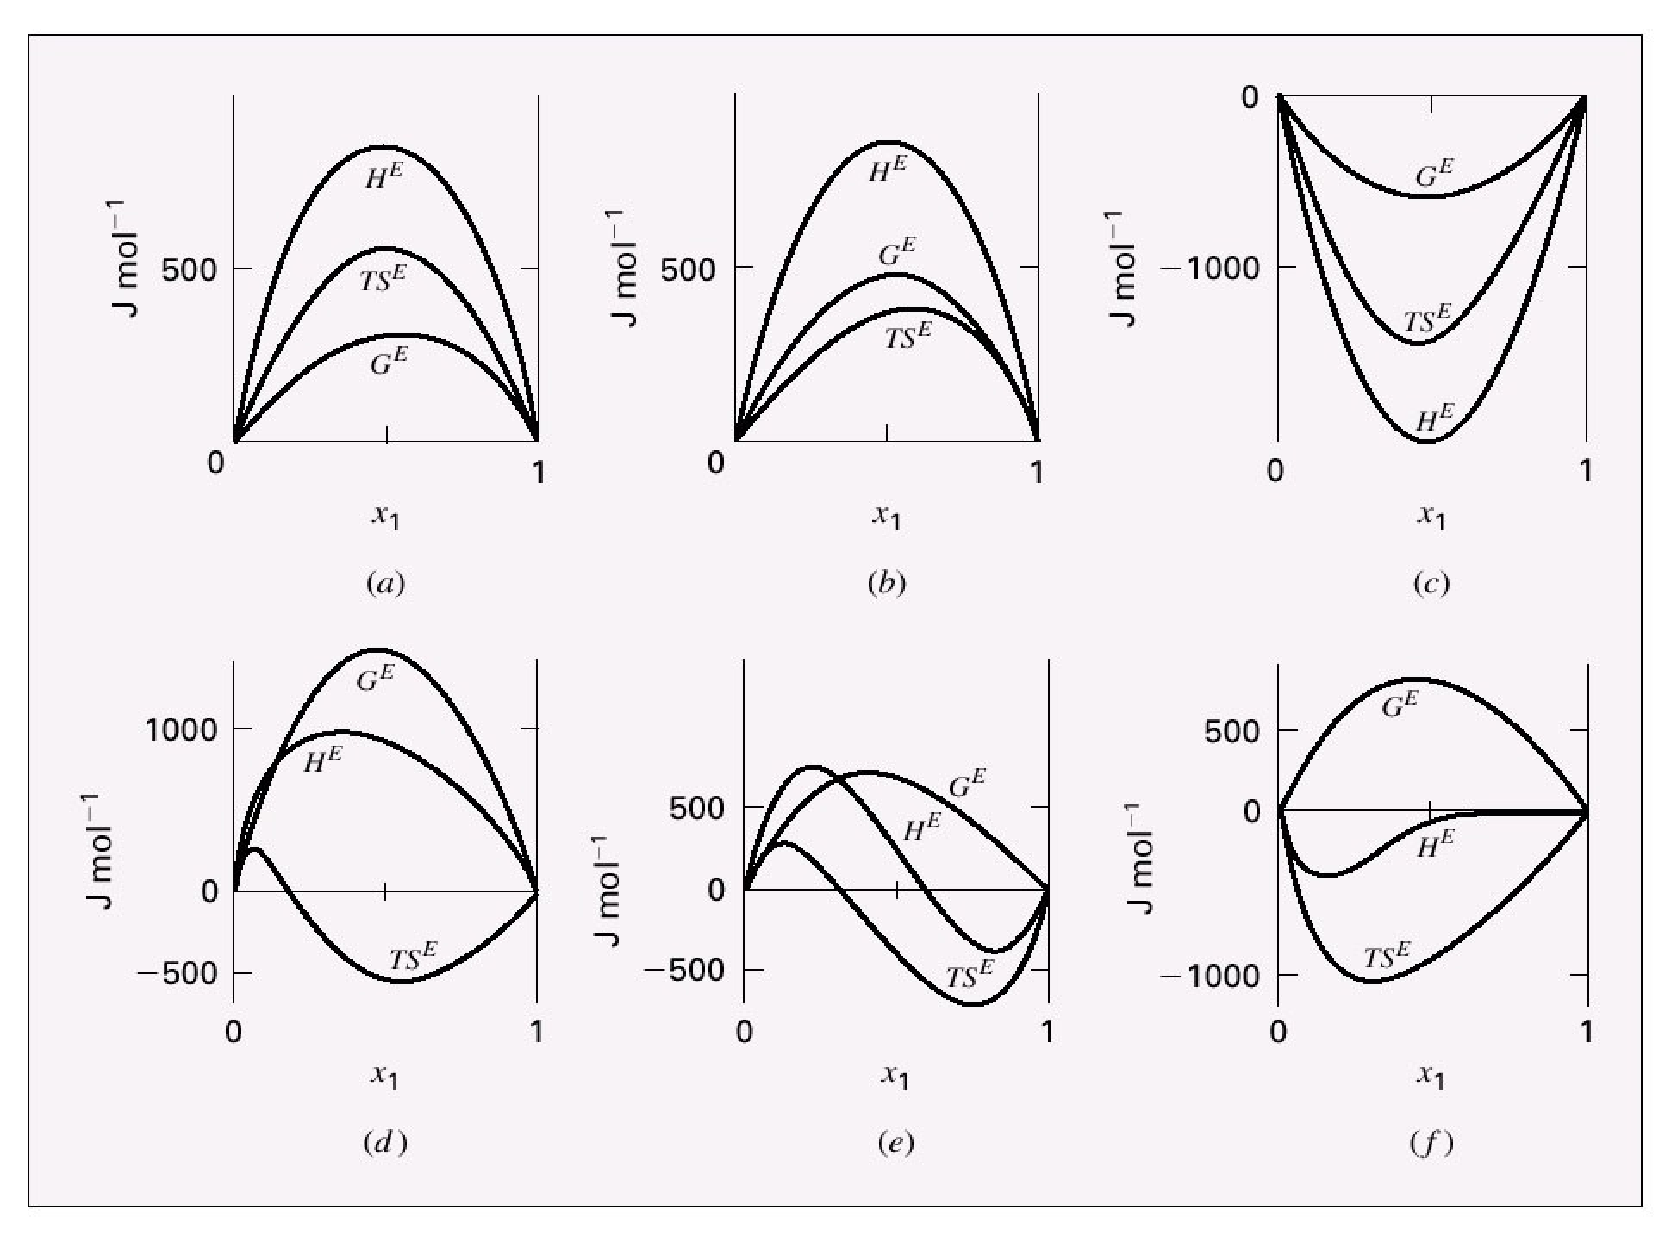
\includegraphics[width=9.cm, height=6.5cm,clip]{./Figs/ExcessProperties_Plot}
          \caption{\scriptsize Excess properties at 50$^{\circ}$C for the following binary liquid systems: (a) chloroform / n-heptane,(b) acetone / methanol, (c) acetone / chloroform, (d) ethanol / n-heptane, (e) ethanol / chloroform and (f) ethanol / water (Extracted from {\it Smith, Van Ness and Abott}). }
       \end{figure}
     \end{center}
\end{frame}
\normalsize

%%%
%%% Slide
%%%
%\scriptsize
\begin{frame}
  \frametitle{Example 1}
    At 25$^{\circ}$C and atmospheric pressure the volume change of mixing of a binary liquid mixture of species $1$ and $2$ is given by,
    \begin{displaymath}
       \Delta V = x_{1}x_{2}\left(45x_{1}+25x_{2}\right)\;\;\;\;\text{ with }\;\;\;\; \left[\Delta V\right] = \frc{cm^{3}}{gmol}
    \end{displaymath}
    with $V_{1}$ = 110 cm$^{3}$.gmol$^{-1}$ and $V_{2}$ = 90 cm$^{3}$.gmol$^{-1}$. Determine the partial volumes, $\overline{V}_{1}$ and $\overline{V}_{2}$ in a mixture containing 40$\%$-mol of species $1$.
      
\end{frame}
\normalsize

%%%
%%% SUBSECTION
%%%
\subsection{Activity Coefficient Models}

%%%
%%% Slide
%%%
%\scriptsize
\begin{frame}
  \frametitle{Activity Coefficient Models}
  \begin{enumerate}%\setcounter{enumi}{8}
      \item<1-> In several industrial and environmental applications EOS can not accurately predict the thermodynamic behaviour of solutions. In these cases, we can estimate the excess Gibbs energy \blue{$G^{\text{E}}$} (see Slide~\ref{ExcessProperty}, item~\ref{activitycoefficient}) by first calculating the activity coefficient, $\gamma_{i}$;
      \item<2-> Activity coefficient models are often more accurate (than traditional EOS) when strong intermolecular interactions are present;
      \item<3-> Models commonly used coefficient activity models in \blue{fluid simulators}:
          \begin{enumerate}
             \item<3-> Margules;
             \item<3-> Van Laar;
             \item<3-> Wilson;
             \item<3-> Non-Random-Two-Liquids (NRTL);
             \item<3-> UNIversal QUAsi Chemical (UNIQUAC).     
          \end{enumerate}
      \item<4-> Basic Equations:
          \visible<4->{\begin{displaymath}
            \gamma_{i} = \frc{\overline{f}_{i}}{x_{i}f_{i}}=\frc{\overline{f}_{i}}{\overline{f}_{i}^{\text{id}}},\hspace{1cm} \frc{G^{\text{E}}}{RT}=\xi\left(\gamma_{i}\right)
          \end{displaymath}
           where $\xi\left(\gamma_{i}\right)$ is a function of $\gamma_{i}$. Bear in mind that $\gamma_{i}$ is a function of composition, $x_{i}$. }
  \end{enumerate}
\end{frame}
\normalsize


%%%
%%% Slide
%%%
%\scriptsize
\begin{frame}
  \frametitle{Activity Coefficient Models}
  \begin{enumerate}\setcounter{enumi}{4}
      \item<1-> 2-parameter models for binary systems:
        \begin{enumerate}
          \item<1-> Mergules equations;
             \visible<1->{\begin{displaymath}
                \ln\gamma_{1}=x_{2}^{2}\left[A_{12}+2\left(A_{21}-A_{12}\right)x_{1}\right] \hspace{1cm} \ln\gamma_{2}=x_{1}^{2}\left[A_{21}+2\left(A_{12}-A_{21}\right)x_{2}\right]
             \end{displaymath}}
          \item<2-> Van Leer equations:
             \visible<2->{\begin{displaymath}
                \ln\gamma_{1}= B_{12}\left(1+\frc{B_{12}x_{1}}{A_{21}x_{2}}\right)^{-2}  \hspace{1cm} \ln\gamma_{2}= B_{21}\left(1+\frc{B_{21}x_{1}}{A_{12}x_{2}}\right)^{-2}
             \end{displaymath}}
          \item<3-> Wilson equations:
             \visible<3->{\begin{eqnarray}
                && \frc{G^{\text{E}}}{RT} = x_{1}\ln\left(x_{1}+x_{2}C_{12}\right) - x_{2}\ln\left(x_{2}+x_{1}C_{21}\right) \nonumber \\
                && \ln\gamma_{1}= -\ln\left(x_{1}+x_{2}C_{12}\right) + x_{2}\left(\frc{C_{12}}{x_{1}+x_{2}C_{12}}-\frc{C_{21}}{x_{2}+x_{1}C_{21}}\right)\nonumber \\
                && \ln\gamma_{2}= -\ln\left(x_{2}+x_{2}C_{21}\right) + x_{2}\left(\frc{C_{12}}{x_{1}+x_{2}C_{12}}-\frc{C_{21}}{x_{2}+x_{1}C_{21}}\right)\nonumber 
             \end{eqnarray}}
        \end{enumerate} 
  \end{enumerate}
\end{frame}
\normalsize


%%%
%%% Slide
%%%
%\scriptsize
\begin{frame}
  \frametitle{Activity Coefficient Models}
  \begin{enumerate}\setcounter{enumi}{5}
      \item<1-> NRTL and UNIQUAC are 3-parameter models that incorporate binary attraction/repulsion parameters of multiple chemical species;
       \item<2-> UNIFAC (UNIQUAC Functional-group Activity Coefficient) is a group contribution model that assign specific thermodynamic properties to functional group species, e.g., \red{$\cdot$CH$_{3}$}, \red{:CH$_{2}$}, \red{:COH}, \red{$\cdot$OH}, etc.
  \end{enumerate}
\end{frame}
\normalsize




\section{Summary}

%%%
%%% Slide
%%%
%\scriptsize
\begin{frame}
 \frametitle{Summary}
   \begin{enumerate}[(i)]
     \item Excess molar properties;
     \item Definition of activity,activity coefficient, fugacity, fugacity coefficient and chemical potential for pure species and mixtures;
     \item Brief description of activity coefficient models currently used in simulators.
   \end{enumerate}
\end{frame}


\end{document}
 
